\documentclass[12pt]{article}
\usepackage[utf8]{inputenc}
\usepackage{mathtools}
\usepackage{amsmath}
\usepackage{hyperref}
\usepackage{wasysym}
\usepackage{mathabx}
\usepackage{float}
\usepackage{xcolor}
\usepackage[numbers,square,super,sort&compress]{natbib} %For a bibliography
\usepackage{cprotect} %For verbatim code in title...
\usepackage{geometry} % Required to change the page size to A4
\usepackage{graphicx,xcolor} %colors and images
\usepackage{subfigure} %useful for multiple figures in one float
\usepackage{amsmath, amssymb} %Mathematical symbols
\usepackage[exponent-product=\cdot, per-mode=symbol]{siunitx} %Useful for physical quantities with units
\usepackage[notrig]{physics} %contains all kinds of useful abbreviations for braket, derivatives, etc.
\usepackage{enumitem,fancyhdr,lastpage,parskip} %For item lists, for headers and footers and no indents
\usepackage[numbers,square,super,sort&compress]{natbib} %For a bibliography
\usepackage[hidelinks]{hyperref}
\usepackage{listings} %Listings package is for scripts
\usepackage{cprotect} %For verbatim code in title...

% CODE ENVIRONMENT
\definecolor{mygreen}{rgb}{0,0.6,0} \definecolor{mygray}{rgb}{0.5,0.5,0.5} \definecolor{mymauve}{rgb}{0.58,0,0.82}
\lstset{basicstyle=\footnotesize, breakatwhitespace=false, breaklines=true, commentstyle=\color{mygreen}, extendedchars=true, frame=single, keepspaces=true, keywordstyle=\color{blue}, language=Python, numbers=left,                    numbersep=5pt, numberstyle=\tiny\color{mygray},  rulecolor=\color{black}, showspaces=false, showstringspaces=false, showtabs=false, stringstyle=\color{mymauve}, tabsize=3, title=\lstname, captionpos=b}
%See for comments for instance here: https://tex.stackexchange.com/questions/83882/how-to-highlight-python-syntax-in-latex-listings-lstinputlistings-command

\textheight=23.5cm
\textwidth=16cm
\oddsidemargin=0cm
\evensidemargin=0cm
\topmargin=-1cm
\parskip=0.2cm
\parindent=0.0cm
\linespread{1.2}

\begin{document}

%----------------------------------------------------------------------------------------
%	TITLE PAGE
%----------------------------------------------------------------------------------------

\begin{titlepage}

\newcommand{\HRule}{\rule{\linewidth}{0.5mm}}

\center
\begin{figure}[H] \center{
\includegraphics[width=0.2\linewidth]{LeidenSeal}} \end{figure}
\textsc{\LARGE Leiden University}\\[1.5cm]


\HRule \\[0.4cm]
{ \huge \bfseries Assignment 1: Questionable Research Practices}\\[0.1cm] % Title of your document
\HRule \\[1.5cm]

\textsc{Author:}\\[0.3cm]
\textsc{\Large Dean Kuurstra (s3343715)}\\[0.5cm]
\textsc{\Large Diego Cañas Jimenez (s3856216)}\\[0.5cm]
\textsc{\Large Koorosh Komeili Zadeh (s3893995)}\\[0.5cm]
\textsc{\Large Lani Hampel (s3977412)}\\[0.5cm]

\large April 18, 2025\\
A Research Methods in Artificial Intelligence report\\
% Date, change the \today to a set date if you want to be precise

\vfill % Fill the rest of the page with whitespace

\end{titlepage}

\newpage
\section{Introduction}
    According to Stanford University Libraries (2023)\cite{rosenfeld2023}, the most common way couples meet is through online dating. This makes online dating a relevant topic of study and interest. To further understand online dating, it is worth considering distinct variables and their effect on the number of matches a user receives. This paper will investigate how the number of previous relationships of a user influences their match rates, and examine the impact of using questionable research practices (QRPs). This may provide further insight into the most common method currently used to find relationships. Furthermore, research into this topic may uncover unknown trends with less obvious features, one of which could be the aforementioned number of previous relationships and a user’s likelihood of successfully finding a match through online dating. \\
    It is interesting to explore the relationship between the number of previous relationships and match rate, as reasonable arguments can defend both (positive and negative) trends. Our study aims to uncover this relationship. For this, we use the number of previous relationships as an explanatory variable, and we use the match rate as the response variable. We aim to examine the relationship through linear regression and thus answer whether the previous number of relationships affects the match rate of the users, whether this effect is positive or negative, if it is indeed present, and how strong this relationship is. 

\section{Hypothesis}
    The Null Hypothesis suggests there is no direct connection between the number of previous significant relationships and the said user's match rate. Thereby, the linear regression’s slope ($\beta$) is zero. The alternative hypothesis suggests that there exists a correlation between the two variables. In other words, $\beta$ is non-zero. Thereby, this is a two-sided test.
    \[
    H_0: \beta = 0
    \]
    \[
    H_a: \beta \neq 0
    \]
    The value of $\alpha$ will be set to 0.05, and therefore any p-value found where $p<0.05$ will be considered significant.

\section{Questionable research practices}
    After analyzing our data, we will implement some QRPs. These QRPs will increase the probability of Type I errors occurring, as they will manipulate the p-value resulting from our linear regression test to more often be below our $\alpha$. First, we will be rounding p-values down to fall below the $0.05$ threshold. In theory, this is effectively the same as increasing $\alpha$ after the data has already been retrieved. Second, we will manipulate p-values by iteratively increasing sample size until a desired p-value is achieved, or until maximum sample size is reached. 

\section{Initial simulation}
\subsection{Data gathering}
    For this project, data for both of our quantitative variables were randomly generated using a normal distribution, partially based on information found online. The standard mean and standard deviation for the normal curve that gives the match are 0.10\cite{elad2024} and 0.15, respectively. The distribution gives the number of previous serious relationships is which breaks the mean of 3 and the standard deviation of 4. The random values that exceeded the limits, namely 0 and 1 for match rate and 0 and 12, were truncated to the closest limit. Ten thousand tests were developed, each containing 5 280 data points. 

\subsection{Findings and analysis}
    A linear regression was drawn for every test, and a slope and p-value were obtained by using the linear regression model. The linear regression model uses a t-test and the standard error. The p-values were then plotted in a histogram with a separation of 0.05.

    \begin{figure}[H]
        \centering
        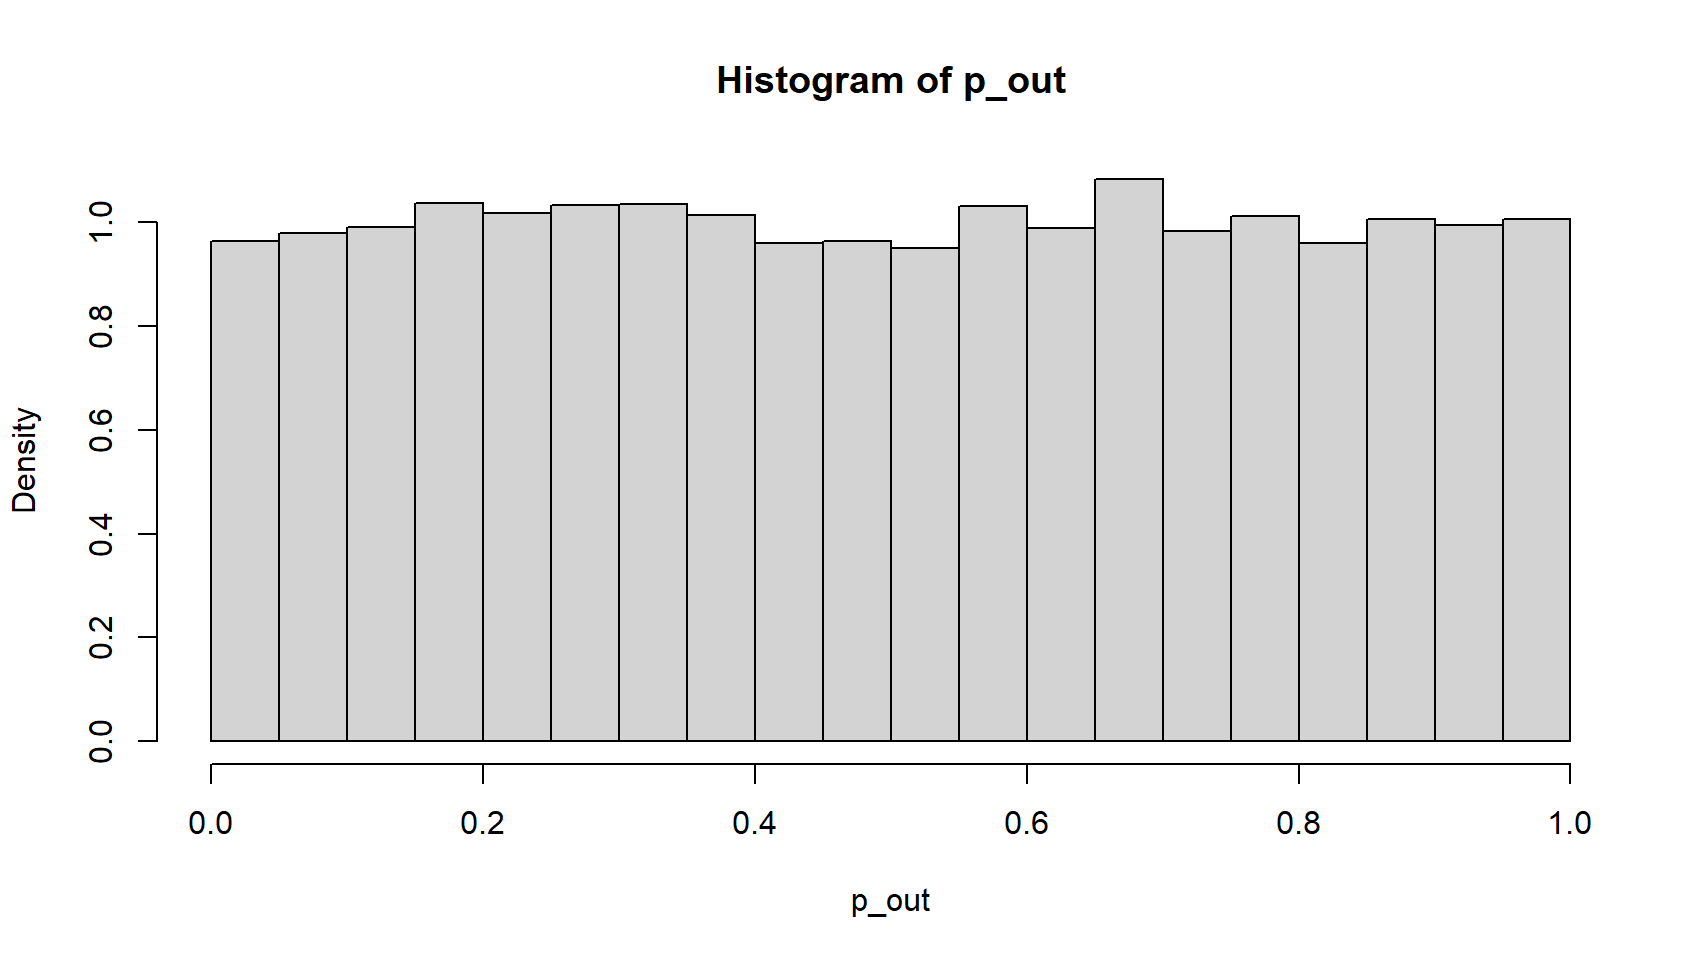
\includegraphics[width=1\linewidth]{figures/R_plotB.png}
        \caption{The histogram shows the distribution of the p-values with their respective densities(related to the frequencies or number of occurrences) in 10 000 tests and a separation of 0.05.}
        \label{fig:enter-label}
    \end{figure}

    Each bin in the histogram represents a range of 0.05 p-values. All bins have a similar probability, namely about 5\%. This value can be obtained by finding the area of the bins. The expected value of false positives for two-sided tests is equivalent the alpha value, namely 0.1, as there are at least two extremes that are as extreme as alpha. The first and last bins represent the false positives as they are at least as extreme as the alpha value (0.05). These extremes give a total area close to 0.1, which approximately matches the expected value.

\section{QRP simulations}
\subsection{P-value rounding}
    This section visualizes the effect of rounding p-values, a questionable research practice, on statistical results. Rounding p-values above 0.05 to 0.05 can increase the number of significant results, increasing false positives and causing inaccurate scientific conclusions to be drawn. It effectively has the same effect as changing the value of $alpha$ after the data has already been gathered to the maximum value that is rounded down the the value of $p$, the former having a value of 0.05 for this report. The following figures show how different maximum rounding values (0.055, 0.06, 0.07, and 0.09) affect the distribution of p-values.

    \begin{figure}[h!]
        \centering
        \begin{minipage}{0.45\textwidth}
            \centering
            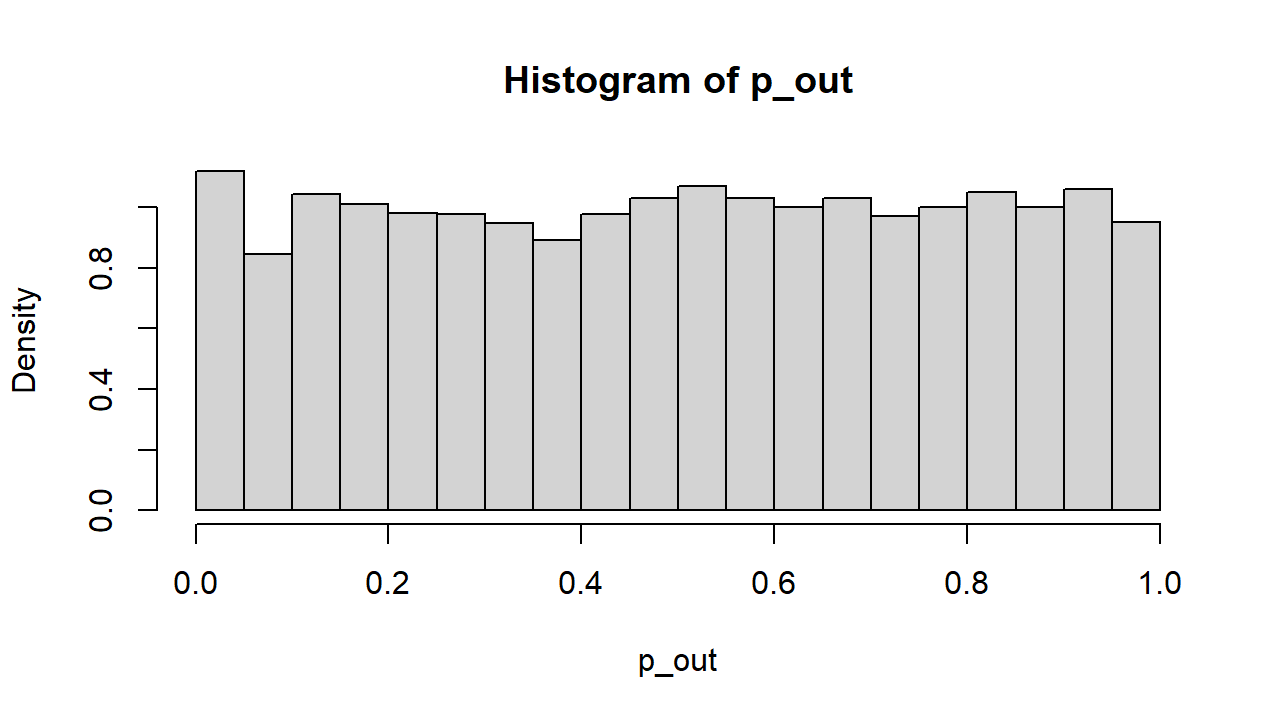
\includegraphics[width=\textwidth]{figures/R_plot_round1.png}
            \caption{Range 0.05 to 0.055 rounded to 0.05}
        \end{minipage} \hfill
        \begin{minipage}{0.45\textwidth}
            \centering
            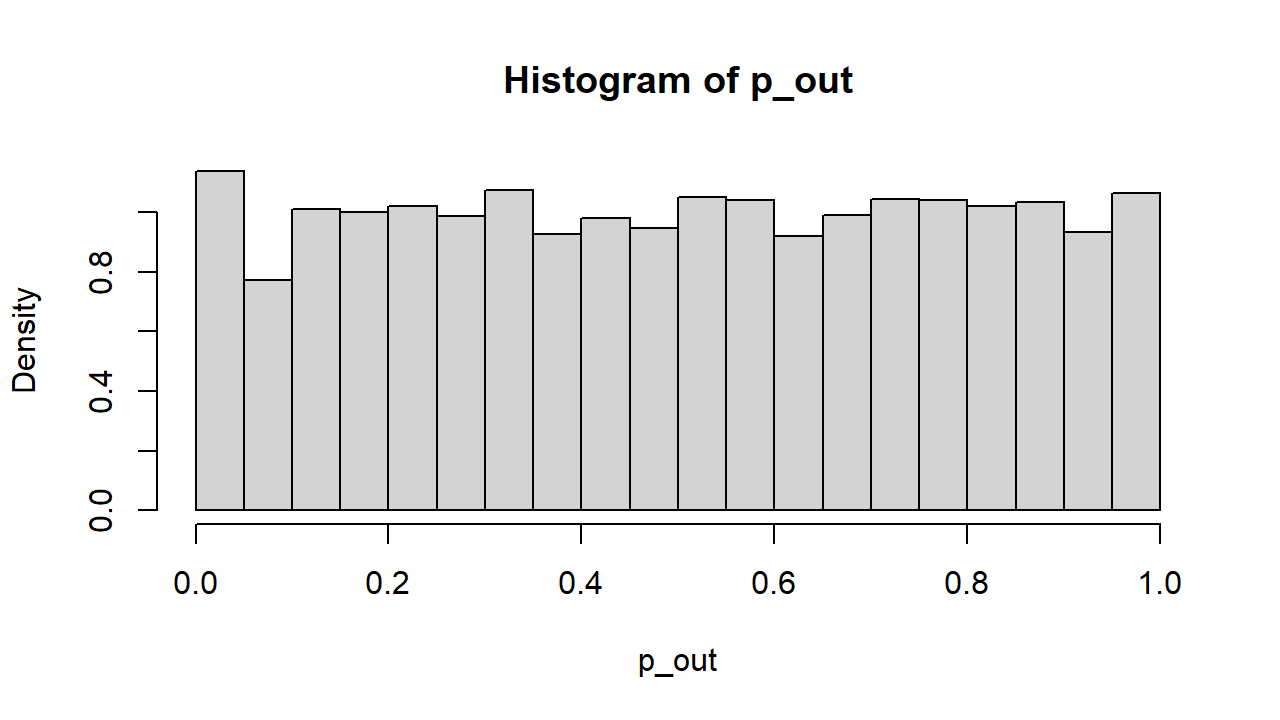
\includegraphics[width=\textwidth]{figures/R_plot_round2.png}
            \caption{Range 0.05 to 0.06 rounded to 0.05}
        \end{minipage}
    
        \vskip\baselineskip
    
        \begin{minipage}{0.45\textwidth}
            \centering
            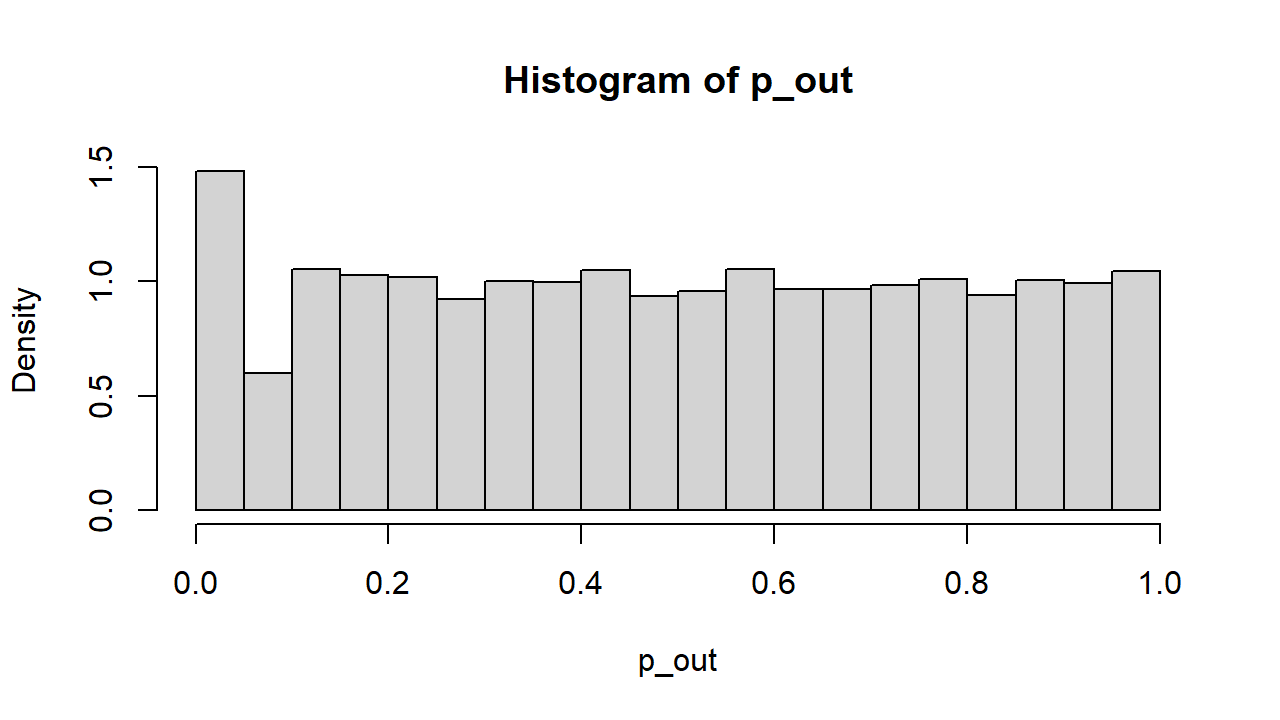
\includegraphics[width=\textwidth]{figures/R_plot_round3.png}
            \caption{Range 0.05 to 0.07 rounded to 0.05}
        \end{minipage} \hfill
        \begin{minipage}{0.45\textwidth}
            \centering
            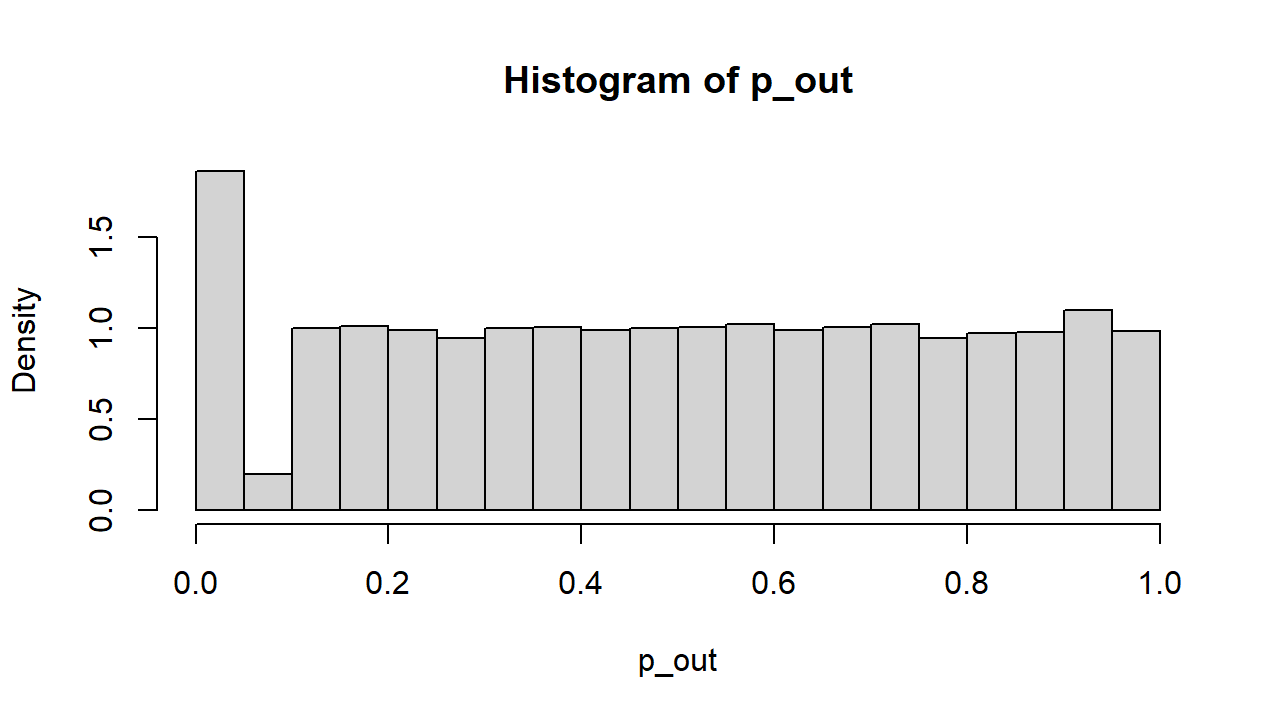
\includegraphics[width=\textwidth]{figures/R_plot_round4.png}
            \caption{Range 0.05 to 0.09 rounded to 0.05}
        \end{minipage}
    \end{figure}

    In the figures, it can be seen that the leftmost bar, which includes all (supposedly) significant p-values, is larger, and the bar directly adjacent to it is smaller. This is because the second bar has a portion of its results rounded down to 0.05, placing it in the first bar instead. If one were to set the maximum rounding value to 0.1, the second bar would be added to the first bar in its entirety. Rounding p-values increases the Type I error rate by making non-significant results, which can cause incorrect replication and have an impact on the reliability and integrity of scientific research. 

\subsection{Sequential testing with optional stopping}
    Another, slightly more complicated way of changing the outcome of a test and manipulating the p-value, is by iteratively adding to the sample size. For this QRP, we initially start with a sample size of $n=280$, after which we iteratively increase the sample size by 200. This increasing of the sample size will occur until we either find that the resulting p-value of the linear regression test is significant ($<0.05$) or when maximum sample size is reached (5 280). If there is no relation between the explanatory and response variable, the p-value will fluctuate randomly when the sample size is increased (though the rate of fluctuation decreases as sample size increases). Therefore, at some point, the p-value of a sample will drop below 0.05 if the sample size is increased forever. In this case, though, we have a limited sample. The following histogram is the result of 10 000 different simulations.

    \begin{figure}[H]
        \centering
        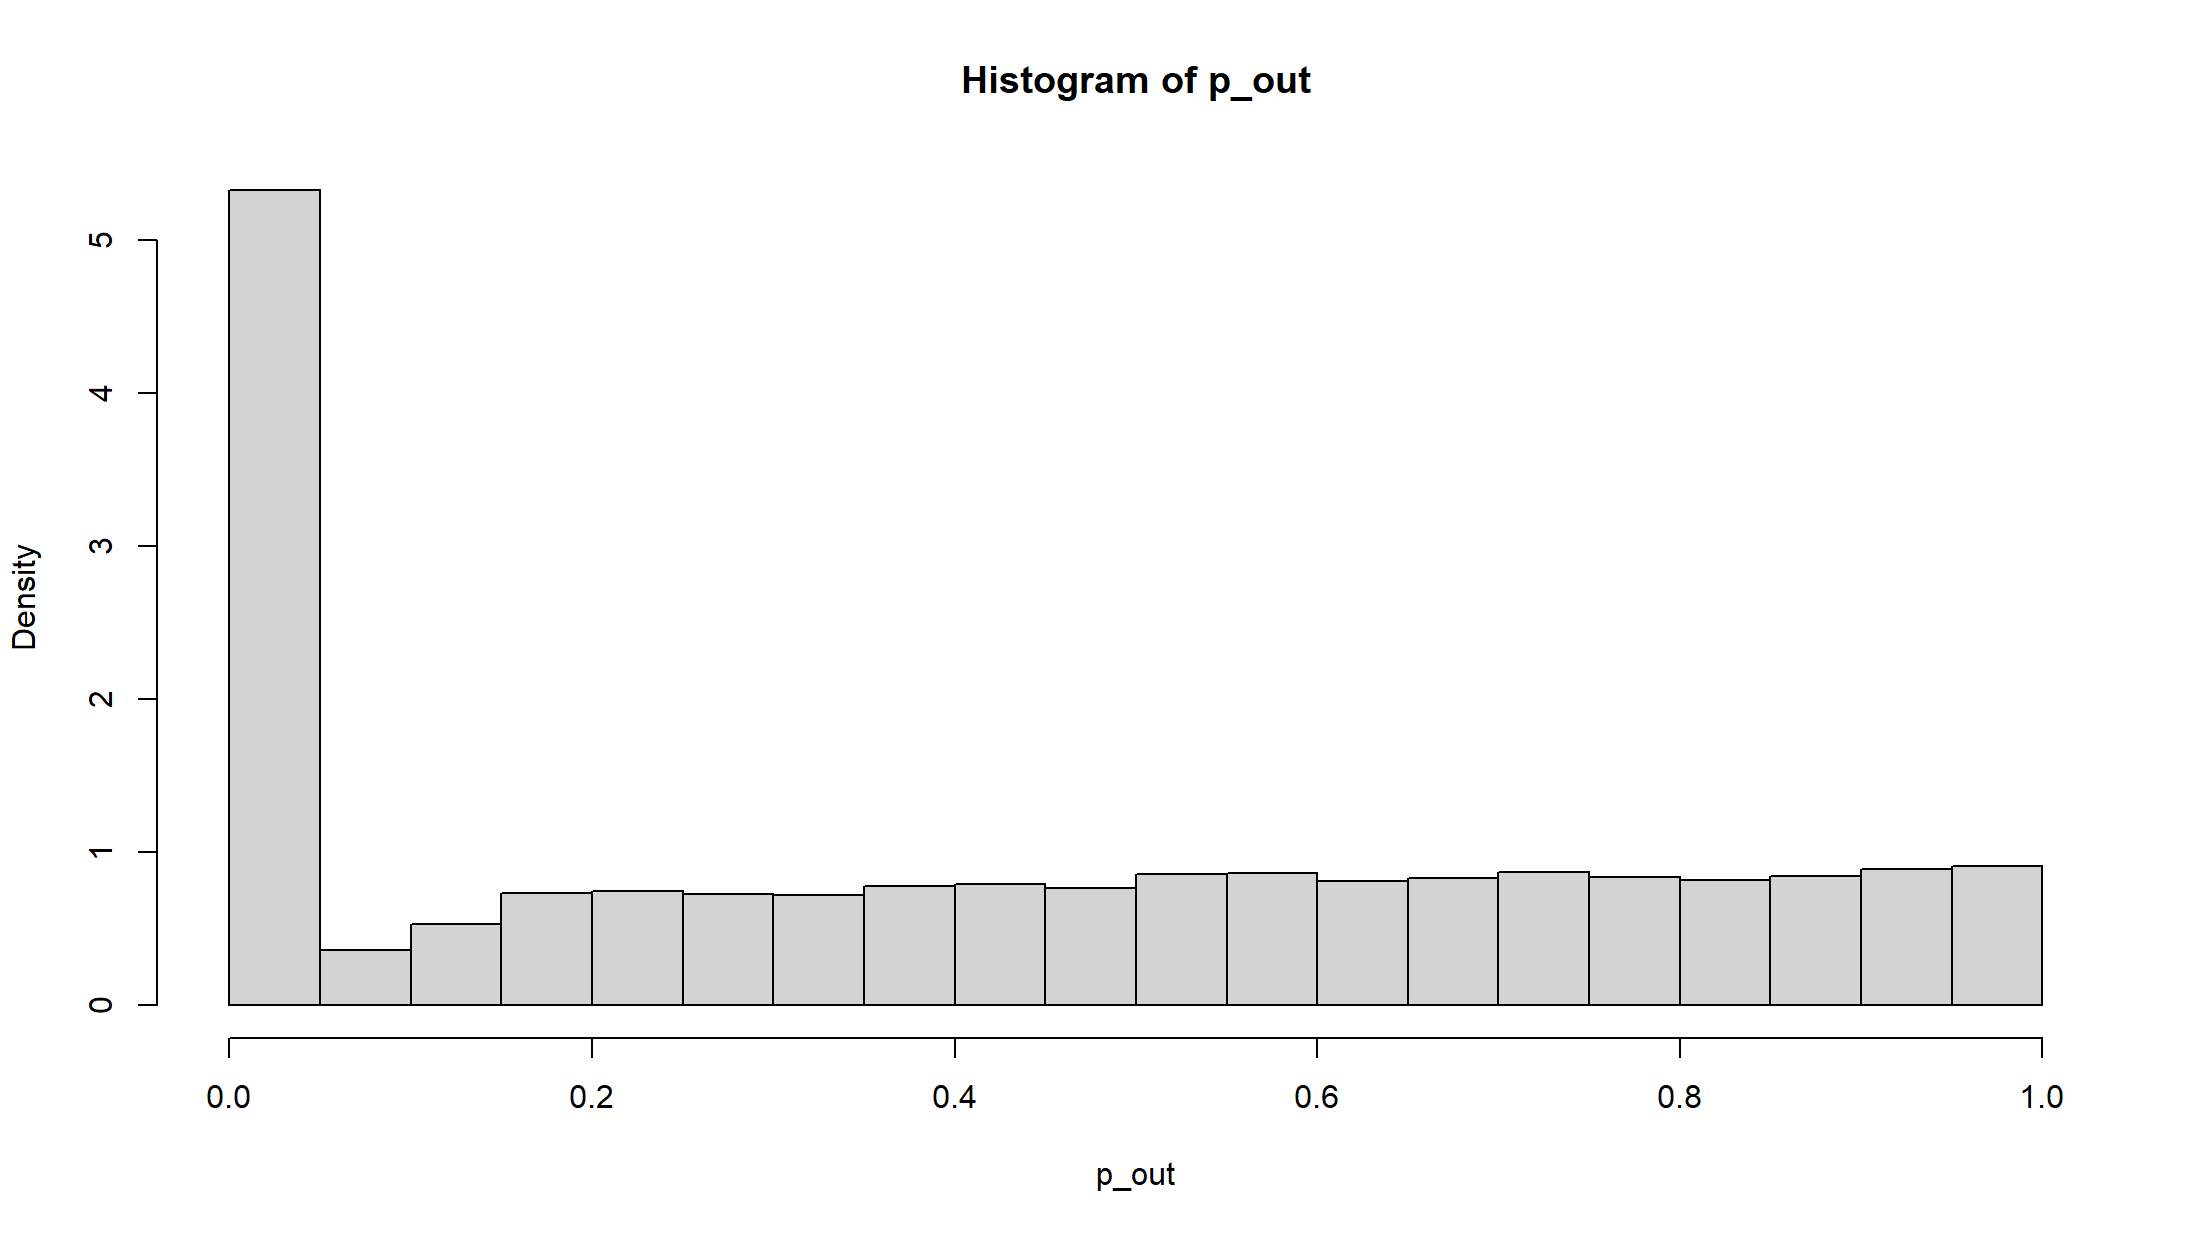
\includegraphics[width=1\linewidth]{figures/R_plot_sequential.png}
        \caption{The histogram shows the distribution of the p-values with their respective densities (related to the frequencies or number of occurrences) in 10.000 tests and a separation of 0.05. The simulation for this figure, though, includes the QRP of sequential testing with optional stopping.}
        \label{fig:enter-label}
    \end{figure}
    
    In the histogram, the leftmost bar is the successfully achieved significant p-values, whereas all the other bars consist of simulations that never achieved a significant p-value. In this histogram, it can also be seen that the bars decrease in size when getting closer to $p=0.05$, as the chance to get to $p<0.05$ somewhere in the sampling increases. These simulations increased the sample size iteratively by 200, but one can also increase it more gradually to capture shorter intervals where $p<0.05$. However, p-values will be very close to 0.05 at most times, as we will recompute $p$ for shorter intervals, and therefore find an earlier moment where the p-value becomes significant. The following graph is a good example to illustrate what is occurring here:

    \begin{figure}[H]
        \centering
        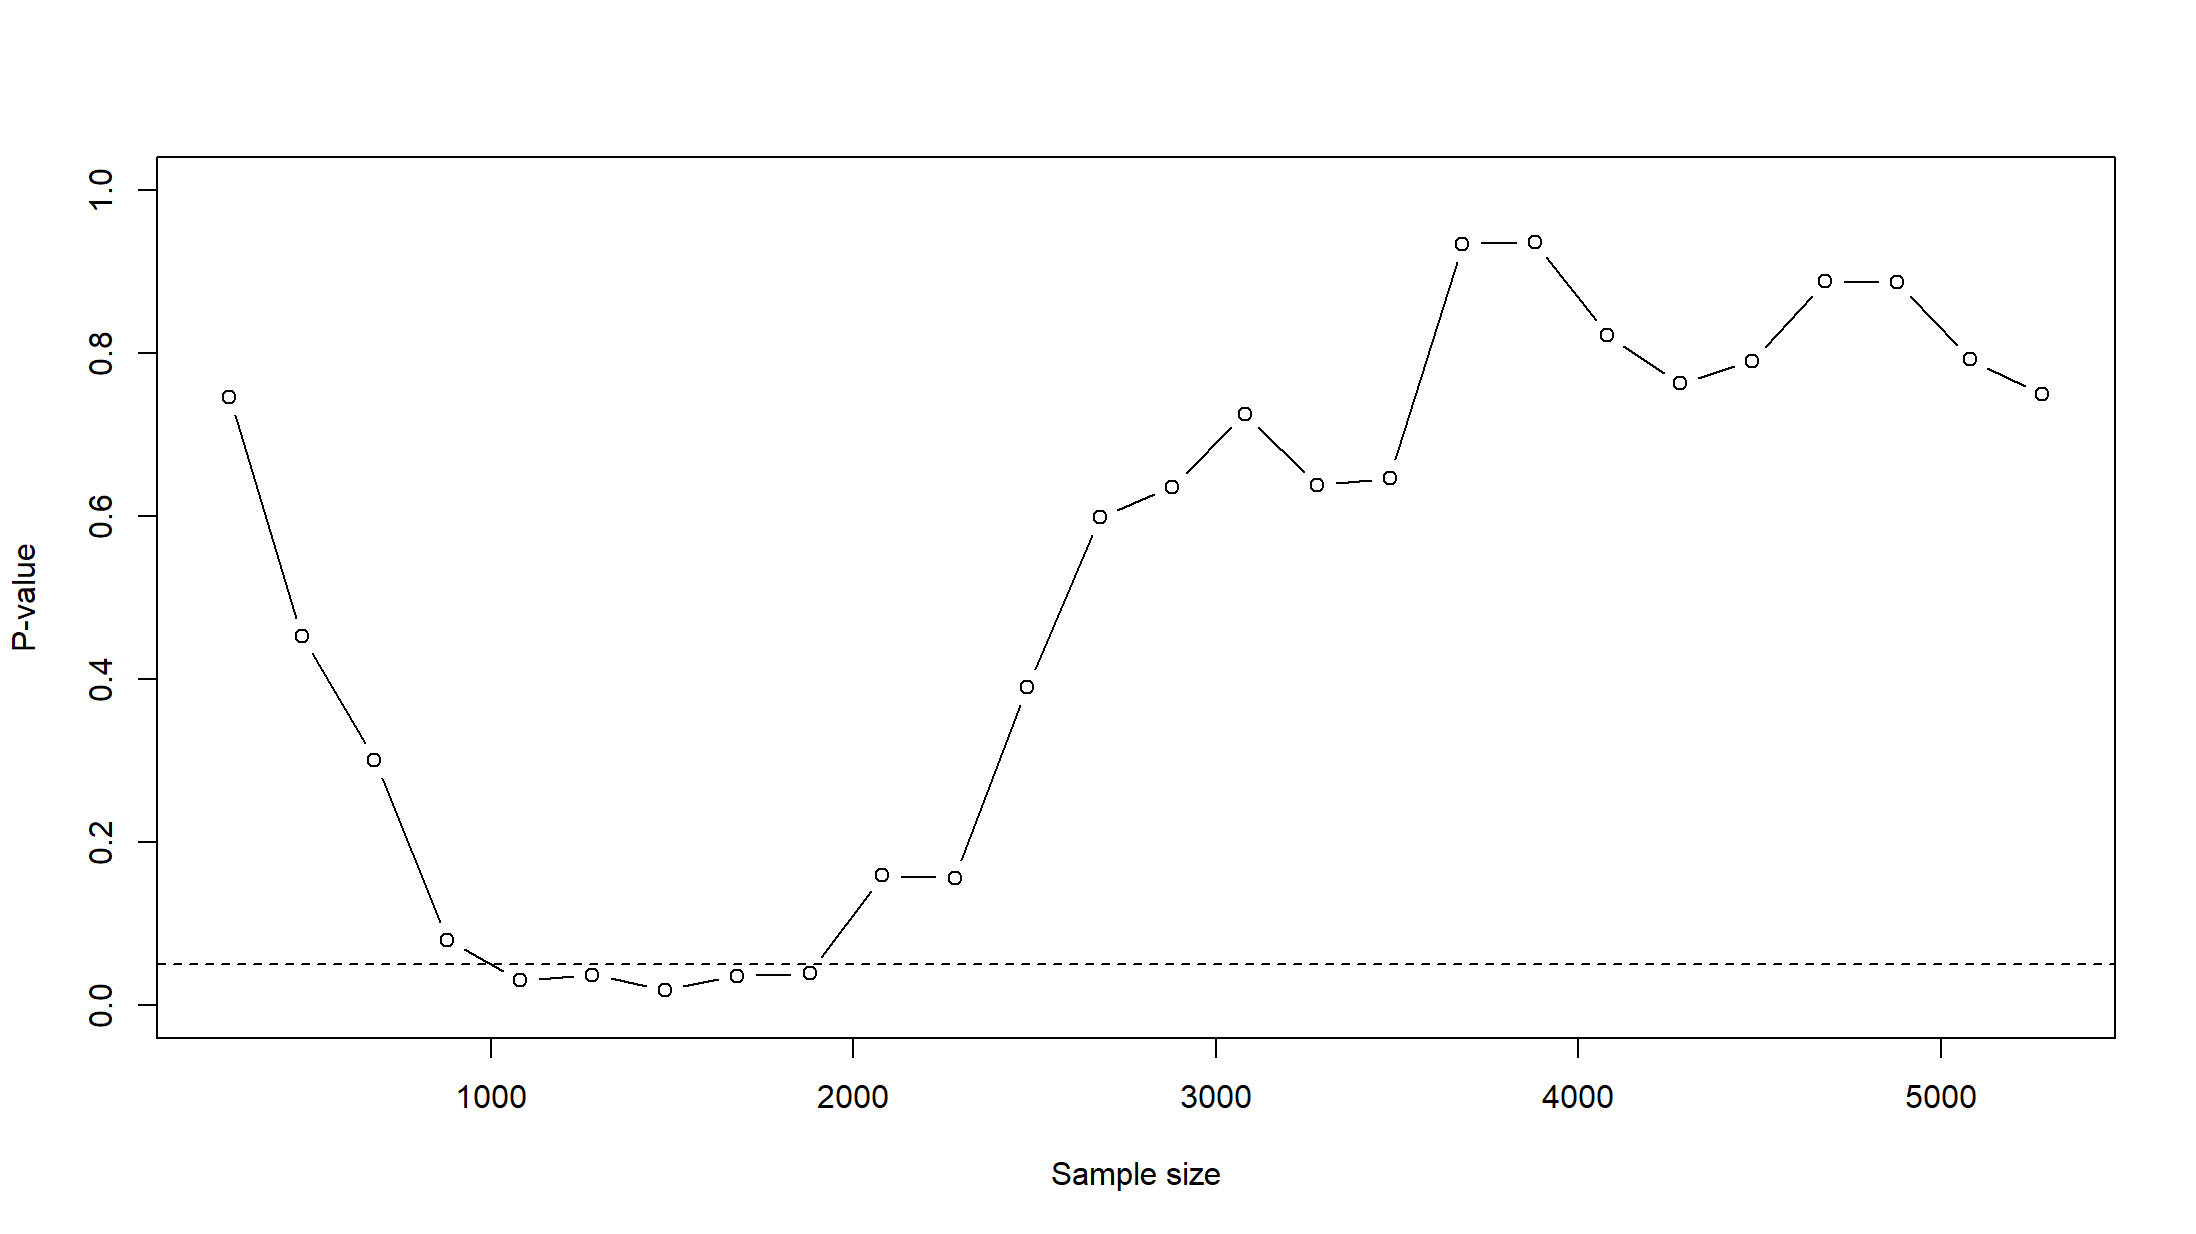
\includegraphics[width=1\linewidth]{figures/R_graph_pval.png}
        \caption{A graph of the p-value of the linear regression test, ran iteratively over a sample size of 5 280.}
        \label{fig:enter-label}
    \end{figure}

    This graph is a very good example of a way we can manipulate the p-value of our simulation. When using this QRP, we first take a sample of 280 people. In the case of Figure 7, this does not retrieve a significant result. We then increase the sample size by 200, adding 200 new data points. We do this iteratively until the horizontal line at $p=0.05$ is crossed. In the case of Figure 7, this happens around 1 000 samples. We then stop sampling and take this p-value as the final p-value.

\section{Conclusion}
    In our dataset, there is no relation between the match rate and number of previous relationships of participants. Therefore, we can conclude that we cannot reject $H_0$. This is clearly visible in Figure 1, where the p-value of 10 000 tests is displayed. The p-values are uniformly distributed, which is what one would expect to see if there is no relation between the explanatory and response variables. \\
    When using our QRPs, though, the p-values tend to group around 0.05. For rounding p-values, this occurs because we simply view any p-value below a certain threshold (but still above 0.05!) to be significant, when in reality, it is not. This results in some results in the second bar partially being grouped into the first bar instead. This QRP is very obvious, and not very effective. It is likely that researchers committing fraud most often do this when they find their observed p-value is very close to the "desired" p-value, and then deciding to fake the observation. \\
    Our second observed QRP, sequential testing with optional stopping, is much more effective. It is less obvious, and dramatically increases the chance of achieving a significant p-value, and in turn tremendously increases the chance of Type I errors as well. This is a much more cunning QRP, as it effectively cannot be discovered by simply looking at the study, or even the dataset. One simply stops gathering samples when the data fits their desired outcome. \\
    For both used QRPs, the probability of a Type I error increases considerably.

\section{Work distribution}
    \begin{itemize}
        \item[] \textbf{Dean Kuurstra}: Introduction (methods), QRP introduction, Initial simulation (R programming), Sequential testing with optional stopping QRP, Conclusion, Report formatting
        \item[] \textbf{Diego Cañas Jimenez}:
        \item[] \textbf{Koorosh Komeili Zadeh}:
        \item[] \textbf{Lani Hampel}:
        \\
    \end{itemize}

\bibliographystyle{ieeetr} 
\bibliography{bibliography}

\end{document}